\let\negmedspace\undefined
\let\negthickspace\undefined
\documentclass[journal]{IEEEtran}
\usepackage[a5paper, margin=10mm, onecolumn]{geometry}
%\usepackage{lmodern} % Ensure lmodern is loaded for pdflatex
\usepackage{tfrupee} % Include tfrupee package

\setlength{\headheight}{1cm} % Set the height of the header box
\setlength{\headsep}{0mm}     % Set the distance between the header box and the top of the text

\usepackage{gvv-book}
\usepackage{gvv}
\usepackage{cite}
\usepackage{amsmath,amssymb,amsfonts,amsthm}
\usepackage{algorithmic}
\usepackage{graphicx}
\usepackage{textcomp}
\usepackage{xcolor}
\usepackage{txfonts}
\usepackage{listings}
\usepackage{enumitem}
\usepackage{mathtools}
\usepackage{gensymb}
\usepackage{comment}
\usepackage[breaklinks=true]{hyperref}
\usepackage{tkz-euclide} 
\usepackage{listings}
\def\inputGnumericTable{}                                 
\usepackage[latin1]{inputenc}                                
\usepackage{color}                                            
\usepackage{array}                                            
\usepackage{longtable}                                       
\usepackage{calc}                                             
\usepackage{multirow}                                         
\usepackage{hhline}                                           
\usepackage{ifthen}                                           
\usepackage{lscape}
\begin{document}

\bibliographystyle{IEEEtran}
\vspace{3cm}

\title{1.3.4}
\author{EE24BTECH11002 - Agamjot Singh
}
% \maketitle
% \newpage
% \bigskip
{\let\newpage\relax\maketitle}

\renewcommand{\thefigure}{\theenumi}
\renewcommand{\thetable}{\theenumi}
\setlength{\intextsep}{10pt} % Space between text and floats

\textbf{Question:}
\newline
If $\vec{A}\brak{1,3}$, $\vec{B}\brak{-1,2}$, $\vec{C}\brak{2,5}$ and $\vec{D}\brak{x,4}$ are the vertices of a parallelogram $ABCD$, then the value of x is
\newline
\textbf{Solution:}
Let $\vec{D}$ be some $\myvec{x\\y}$.
By parallelogram law of addition, 
\begin{align}
	\vec{BA} + \vec{BC} &= \vec{BD}\\
	\vec{BA} &= \vec{A} - \vec{B} = \myvec{1\\3} - \myvec{-1\\2} = \myvec{2\\1}\\
	\vec{BC} &= \vec{C} - \vec{B} = \myvec{2\\5} - \myvec{-1\\2} = \myvec{3\\3}\\
	\vec{BD} &= \vec{D} - \vec{B} = \myvec{x\\y} - \myvec{-1\\2} = \myvec{x+1\\y-2}\\
	\text{By equation (1), you get}\\
	\myvec{x+1\\y-2} &= \myvec{2\\1} + \myvec{3\\3} = \myvec{5\\4}\\
	x &= 4, y = 6
\end{align}

By equation $\brak{7}$, we can see that no such $\vec{D}$ in the form $\myvec{x\\4}$ exists.


\begin{figure}[h!]
   \centering
   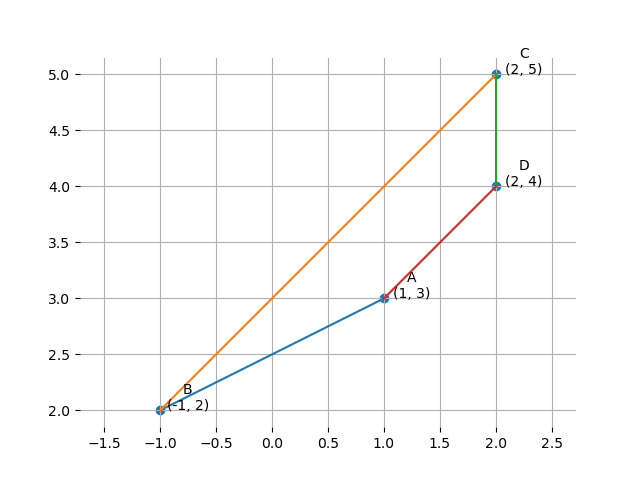
\includegraphics[width=0.7\linewidth]{figs/graph.png}
   \caption{Quadrilateral ABCD formed with given equations}
   \label{label}
\end{figure}

\end{document}
